\documentclass{article}

% if you need to pass options to natbib, use, e.g.:
% \PassOptionsToPackage{numbers, compress}{natbib}
% before loading nips_2018

% ready for submission
%\usepackage{nips_2018}

% to compile a preprint version, e.g., for submission to arXiv, add
% add the [preprint] option:
\usepackage[preprint]{nips_2018}

%\usepackage[square,numbers]{natbib}
\bibliographystyle{unsrt}


% to compile a camera-ready version, add the [final] option, e.g.:
% \usepackage[final]{nips_2018}

% to avoid loading the natbib package, add option nonatbib:
%\usepackage[nonatbib]{nips_2018}

\usepackage[utf8]{inputenc} % allow utf-8 input
\usepackage[T1]{fontenc}    % use 8-bit T1 fonts
\usepackage{hyperref}       % hyperlinks
\usepackage{url}            % simple URL typesetting
\usepackage{booktabs}       % professional-quality tables
\usepackage{amsfonts}       % blackboard math symbols
\usepackage{nicefrac}       % compact symbols for 1/2, etc.
\usepackage{microtype}      % microtypography
\usepackage{graphicx}

\title{CycleFlow: Project Progress Report}

% The \author macro works with any number of authors. There are two
% commands used to separate the names and addresses of multiple
% authors: \And and \AND.
%
% Using \And between authors leaves it to LaTeX to determine where to
% break the lines. Using \AND forces a line break at that point. So,
% if LaTeX puts 3 of 4 authors names on the first line, and the last
% on the second line, try using \AND instead of \And before the third
% author name.

\author{
  Alex Kolchinski\\
  \texttt{yakolch@stanford.edu}\\
  \And
  Andrew Kondrich\\
  \texttt{andrewk1@stanford.edu}\\
}

\begin{document}
% \nipsfinalcopy is no longer used

\maketitle
\section{Introduction}
\subsection{Problem and related work}
Image-to-image translation is the task of mapping images between two image domains, like mapping a landscape painting to a photographic representation of the same scene or vice-versa. In the supervised setting, where training data includes labeled pairs of images, systems like pix2pix \citep{isola2017image} have achieved great success in learning domain-to-domain mappings. More recently, promising results have been demonstrated in the unsupervised setting as well, where only unpaired samples are available from the two domains which the system must learn to map between \citep{zhu2017unpaired, yi2017dualgan, kim2017learning}. These models generally take an approach with paired GANs \citep{goodfellow2014generative}, where in a setting with two domains, each of the two generators learns one of the two mapping directions, and each of the two discriminators learns to discriminate generated samples from training data for one of the two domains. 

While these models achieve good results, they have the drawback of intractable likelihoods, which is inherent to GANs \citep{kingma2018glow}. This also means that the training of such adversarially-trained models is less stable than could be achieved by training by maximum likelihood. Another drawback of the paired-GAN approach used in CycleGAN \citep{zhu2017unpaired} is that the cycle consistency loss, which encourages the two generators to learn inverse mappings of each other, actually induces steganographic behavior which discourages the generators from becoming inverses of each other and affects sample quality \citep{chu2017cyclegan}. 

Flow-based models offer an avenue to addressing these limitations. Over the last few years, models like NICE \citep{dinh2014nice}, Real NVP \citep{dinh2016density} and Glow \citep{kingma2018glow} have made great progress in flow-based generative models, which learn a fully invertible mapping between a latent space with tractable likelihood estimation and sampling and the space of the data. While these models have historically been used for mapping between a data distribution and a latent space, here we demonstate a model that learns a similar invertible mapping to map between two domains in a fully reversible way, alleviating many of the drawbacks of the paired-GAN style models. 

Moreover, our use of a mapping which is both invertible and has tractable determinants means that the subsequent step of learning a mapping to a shared latent space with tractable likelihoods and sampling for two paired domains should be a direct next step, allowing not only the usual advantages of single-domain models with tractable likelihoods but also encouraging the shared latent space to learn semantically meaningful disentangled representations, which would be necessary for the inter-domain mapping to be learned in the unsupervised setting.

\subsection{Plan of Approach}
We have already put together a preliminary model which replaces the paired generators in CycleGAN \citep{zhu2017unpaired} with the two directions of an invertible NICE transform \citep{dinh2014nice}. On 64x64 cropped images from the map2sat database, a very small model (all we had time to test for now) begins to learn a mapping between the satellite image and map domains, while doing quite well on the identity property (maps fed through the sat->map direction should remain unchanged) and perfectly on the cycle consistency by the nature of the model.

While the current results are far from good, this is to be expected from the weak model we are using, and we will proceed by:
\begin{itemize}
    \item Replacing channel shuffling with invertible 1x1 convolutions as in Glow \citep{kingma2018glow}
    \item Implementing Gaussianized splitting out of half of the variables at every coupling layer step as in Real NVP \citep{dinh2016density} and Glow \citep{kingma2018glow}
    \item Adding affine coupling layers as in Real NVP \citep{dinh2016density} (currently we are using additive coupling layers as in NICE \citep{dinh2014nice})
\end{itemize}
All of these steps are expected to substantially increase the power of our model and improve our results.

We will also conduct architecture/hyperparameter search to find the optimal settings for the domains which we will work with, allowing for the computational constraints we are under. We will also experiment with variations to the Glow architecture which will reduce the computational requirements per model size, e.g. weight sharing across coupling layers.

We plan to report final results on the Cityscapes \citep{Cordts2016Cityscapes} dataset, as that is the main benchmark data for CycleGAN. After tuning the architecture and parameters to achieve good generated samples, we will evaluate quality metrics on our samples relative to the CycleGAN model. 

After achieving good quality when mapping between two domains, we plan to investigate learning a shared latent space as well, by introducing a Glow-style maximum likelihood objective in which the two domains are both mapped through invertible mappings with tractable determinants to a shared latent space Z, such that $Z = G(X), Y = F(X), Y = F(G^{-1}(Z))$. Training this model with maximum likelihood, possibly with an auxiliary adversarial objective for sample quality as in FlowGAN \citep{grover2017flow}, should yield more stable training behavior than the dual-GAN approach, in addition to tractable likelihoods and a latent space which is forced to learn a semantically disentangled representation of the two domains by the requirement of learning a semantically paired representation of the two domains simultaneously.

\section{Problem Statement}
\subsection{Dataset}
We begin with cropped and scaled map2sat for quick iteration, and intend to move to full-scale map2sat and Cityscapes-to-semantic labels.

\subsection{Expected Results}
Relative to CycleGAN, we posit that there will be fewer or even no steganographic artifacts in our samples due to our use of an invertible generator, which does not require an explicit cycle consistency loss to train. We expect that this will yield higher sample quality. 
\subsection{Evaluation}
Our quantitative evaluation will be focused on the Cityscapes dataset, which is the main evaluation dataset used in CycleGAN. We will evaluate our model's performance based on FCN score \citep{isola2017image}, which evaluates how well our generated samples correspond to a pre-trained segmentation network. We will also use other Cityscapes metrics such as per-pixel accuracy, and mean class IOU. We also intend to include a Frechet Inception Distance (FID) score \citep{heusel2017gans} for all datasets used. We hope to test for the amelioration of steganography in our samples using techniques described in  \citep{chu2017cyclegan}, such as observing samples modified with adaptive histogram equalization. 
\section{Technical Approach}
Given two domains $X$ and $Y$, our goal is to learn a bidirectional generation function $F: X \rightarrow Y$ where F is invertible such that $F^{-1}: Y \rightarrow X$. We learn this function adversarially through the use of two discriminators, $D_X$ and $D_Y$, where given  $y \in Y$ and $x \in X$, $D_X$ learns to distinguish real samples $x$ from generated samples $F(y)$, and $D_Y$ learns to distinguish real samples $y \in Y$ from generated samples $F(x)$. We include an identity loss term such that $F(y) \approx y$ and $F^{-1}(x) \approx x$.

Our loss $$\mathcal{L} = \mathcal{L}_{GAN} + \mathcal{L}_{idt}$$ is composed of the GAN loss $$\mathcal{L}_{GAN} = \mathbb{E}_{y\sim p_{data}(y)}[\log D_Y(y)] + \mathbb{E}_{x\sim p_{data}(x)}[\log (1 - D_Y(F^{-1}(x)))]$$

And the identity loss 
$$\mathcal{L}_{idt} = \ell_1(X, F^{-1}(Y)) + \ell_1(Y, F(X))$$

This is similar to the formulation in CycleGAN \citep{zhu2017unpaired}, except that we do not require a cycle consistency loss as our model is automatically cycle-consistent.

Our generator is composed of a sequence of additive coupling layers, optionally with squeezing layers interposed, as in NICE \citep{dinh2014nice} and Real NVP \citep{dinh2016density}. This will be augmented later as mentioned above.
The discriminators, as in CycleGAN, are PatchGANs \citep{isola2017image}.

\section{Preliminary Results}

\begin{figure}[h]
\centering
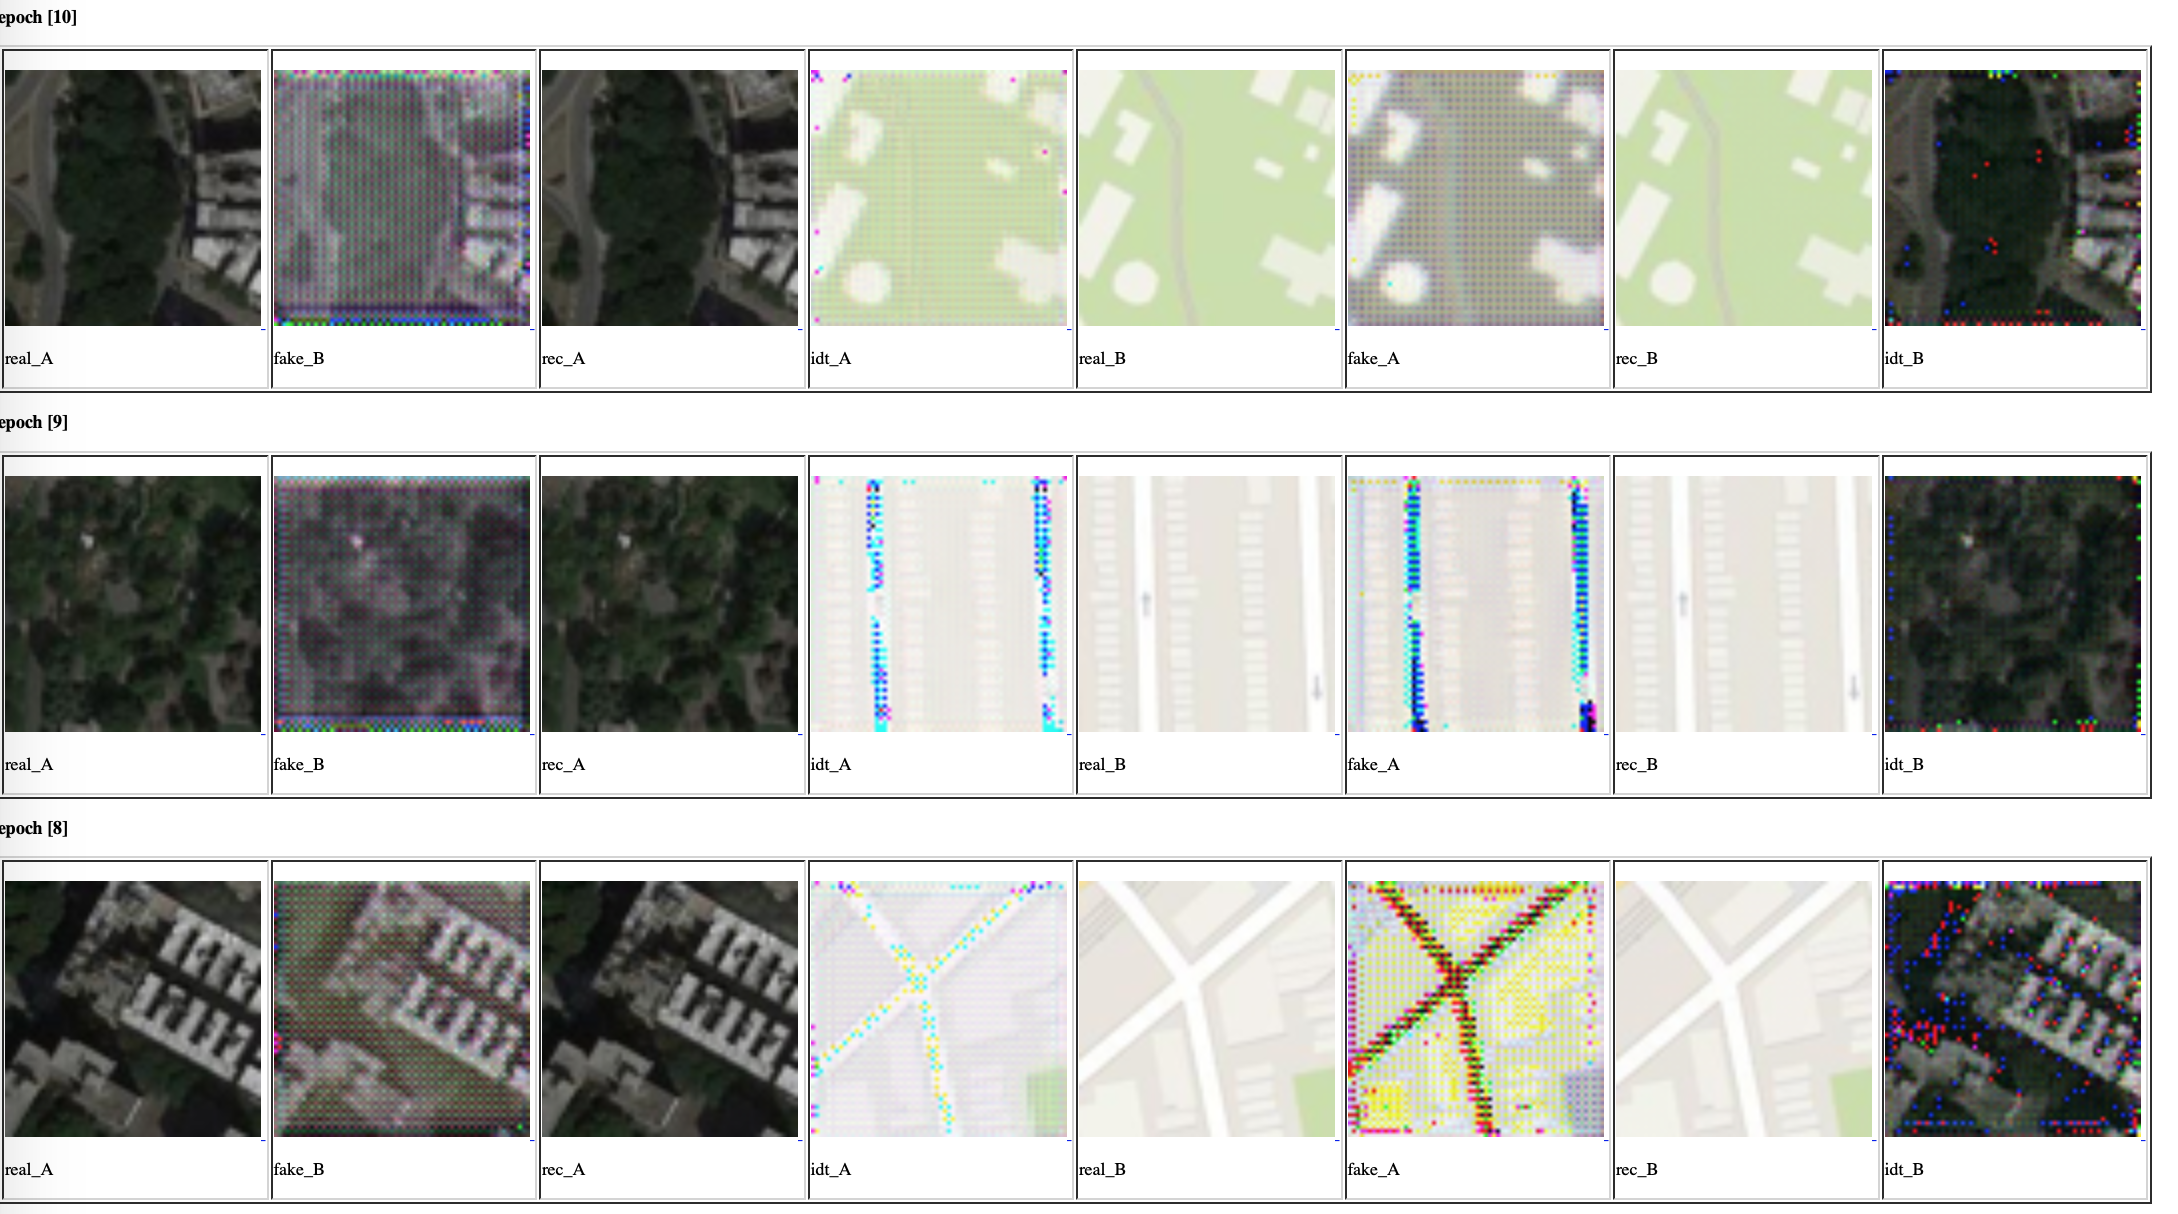
\includegraphics[width=0.9\textwidth]{results.png}
\caption{Sample results}
\end{figure} 

Please see the enclosed figure for a representative example of our current performance. The model is implicitly cycle-consistent by nature, so the rec\_A and rec\_B images created by mapping an image first through one direction of the generator and then through the other (the inverse of the first) are perfect. The model also learns quite quickly to respect the identity loss and keep images largely unchanged when mapped in reverse through the generator. The model also begins to learn to map characteristics of the two domains from one to each other in the fake\_A and fake\_B images, but clearly the results are far from perfect. We expect that a combination of larger models, more powerful architecture as described above, and longer training will yield better results.

\bibliography{main}

\appendix
\end{document}
